% vim: set spell spelllang=es syntax=tex :

\documentclass[11pt,a4paper,spanish]{beamer}

\usepackage[spanish]{babel}

\usepackage[utf8]{inputenc}

\usepackage{graphicx}

\usepackage{subcaption}

\usepackage{url}

\usepackage{lineno} \linenumbers

\usepackage{babelbib}

\setlength{\parskip}{1.5mm}

\usetheme{Rochester}

\usecolortheme{whale}

\beamertemplatenavigationsymbolsempty

\setbeamertemplate{background canvas}{
	\raisebox{-0.99\paperheight}[0pt][0pt]{
	\makebox[\paperwidth]{
		\null
		\hspace{0.9\paperwidth}
		\hspace{-2em}
		\includegraphics[width=0.1\paperwidth]{logos/uncoma.pdf}
		}
	}
}

\title{Un sistema paralelo de visión global para fútbol de robots
	orientado al uso educativo}

\author{}

\date{}

\begin{document}

\begin{frame}

	\maketitle

\begin{itemize}

	\item Autor: Cañibano, Rodrigo \texttt{<rcanibano@\footnote[1]{fi.uncoma.edu.ar}>}

	\item Director: Balladini, Javier \texttt{<javier.balladini@\footnotemark[1]>}

	\item Codirector: Grosclaude, Eduardo \texttt{<eduardo.grosclaude@\footnotemark[1]>}

\end{itemize}

\end{frame}

\begin{frame}

\begin{itemize}

\item Introducción:

\begin{itemize}

	\item ¿Que es un sistema de visión global para fútbol de robots?

	\item ¿Por que un sistema con fines educación?

	\item ¿Por que paralelo?

\end{itemize}

\item Descripción del sistema:

\begin{itemize}

	\item Oportunidades de paralelismo.

	\item División de los datos.

	\item Arquitectura del sistema.

	\item Experimentación y resultados.

	\item Uso educativo.

\end{itemize}

\item Conclusiones y trabajos futuros

\end{itemize}

\end{frame}

\begin{frame}

\frametitle{¿Que es fútbol de robots?}

	Nos enfocamos en la liga de tamaño pequeño \emph{SSL} de la
	\emph{RoboCup}:

\begin{itemize}

	\item Dos equipos de seis robots cada uno.

	\item Una computadora por equipo controla los robots.

	\item Sistema de visión global (\emph{SVG}) compartido por ambos
		equipos.

\end{itemize}

\end{frame}

\begin{frame}

\frametitle{Arquitectura del \emph{SVG} para la \emph{SSL}}

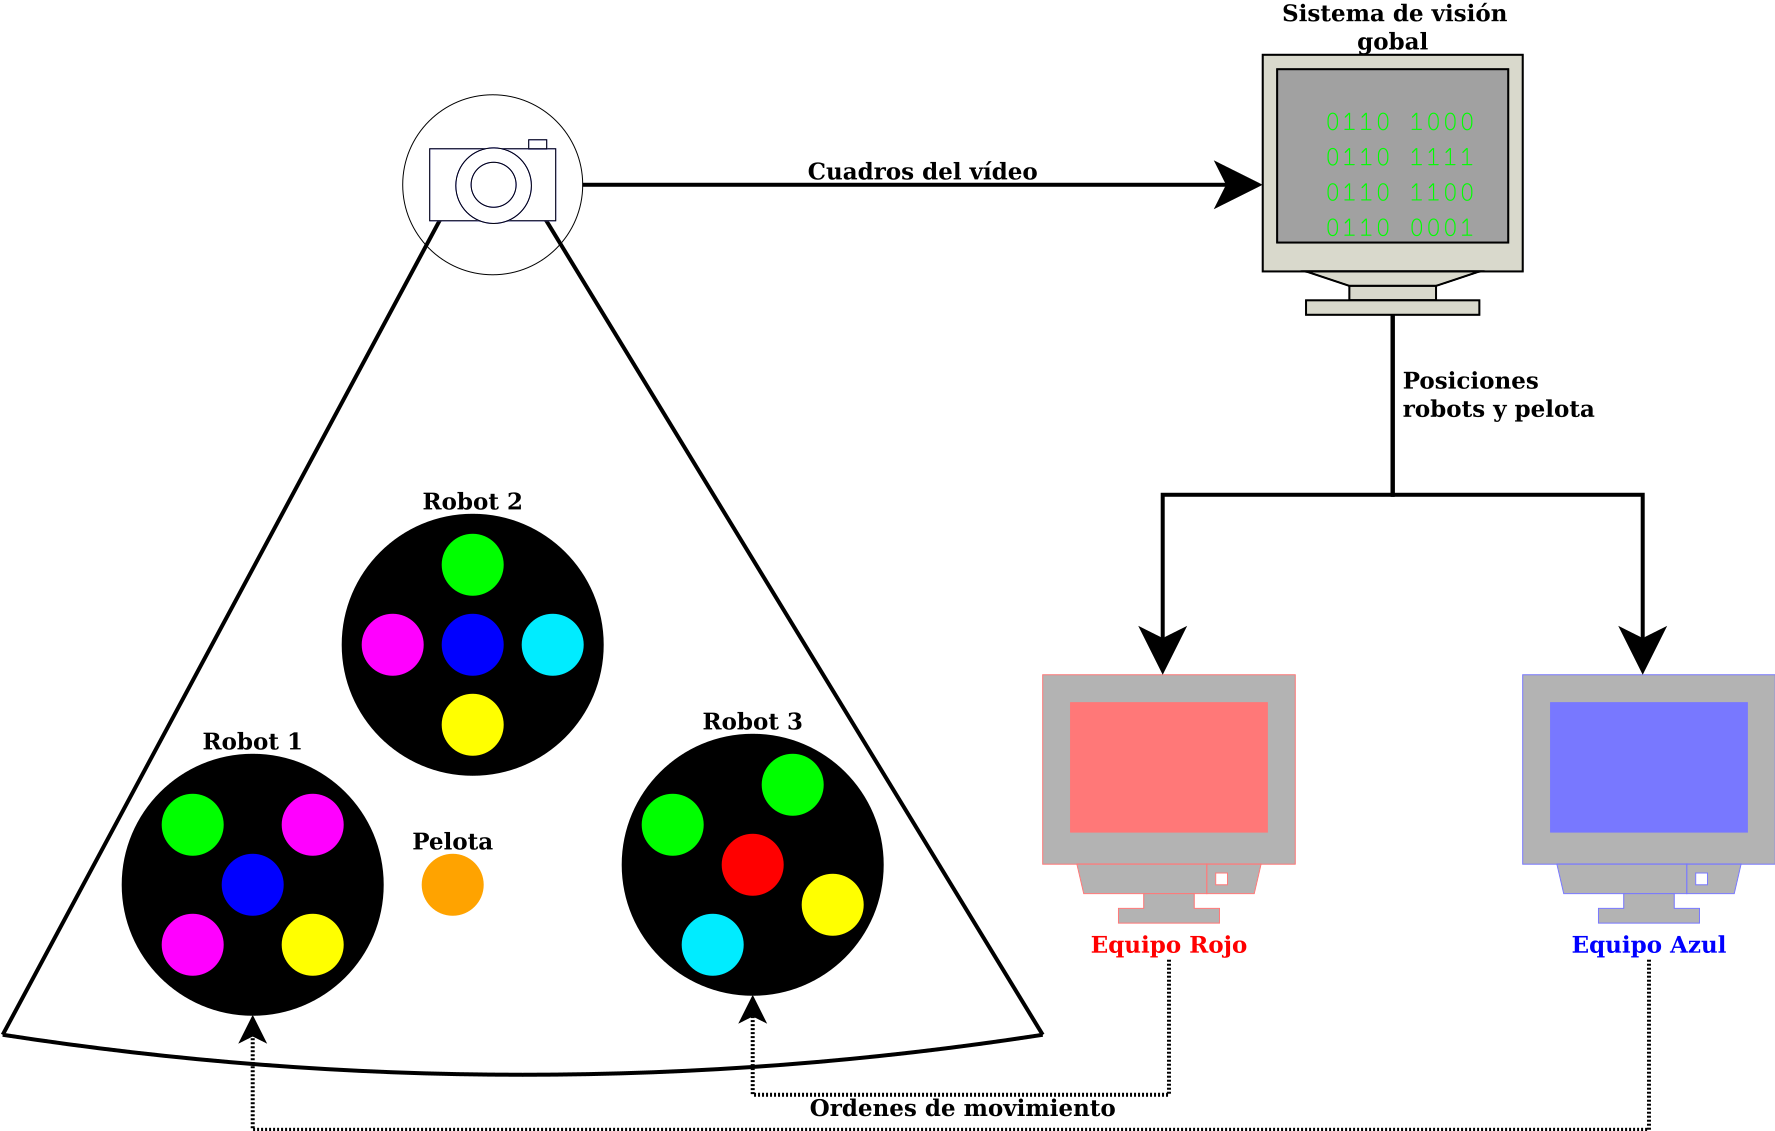
\includegraphics[width=\textwidth]{img/sistemaVG.pdf}

\end{frame}

\begin{frame}

\frametitle{Distribución Arquitectura de las cámaras en un partido de la \emph{SSL}}

\begin{figure}[h]

	\centering

	\begin{subfigure}[c]{0.40\textwidth}
		\centering
		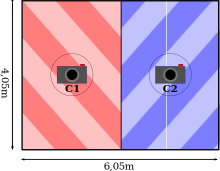
\includegraphics[scale=0.5]{img/cancha605cm.pdf}
		\caption{}
	\end{subfigure}
	~
	\begin{subfigure}[c]{0.40\textwidth}
		\centering
		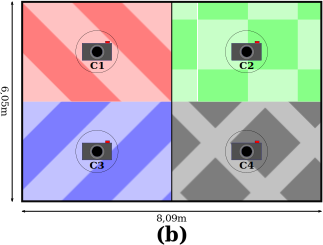
\includegraphics[scale=0.5]{img/cancha809cm.pdf}
		\caption{}
	\end{subfigure}

\end{figure}

\end{frame}

\begin{frame}

\frametitle{Software de \emph{SVG} de la \emph{SSL}}

\begin{itemize}

	\item Problema ideal para la introducción a la visión por computadora.

\end{itemize}

Pero:

\begin{itemize}

	\item Para la \emph{RoboCup} el \emph{SVG} es un problema ya
		solucionado: \emph{SSL-VISION}

	\item \emph{SSL-VISION}: plugins muy avanzados para su uso como
		herramienta educativa.

	\item El sistema actual no es escalable, pero el tamaño de la cancha
		sigue aumentando.

\end{itemize}

\end{frame}

\begin{frame}

\frametitle{Objetivos}

Desarrollar un \emph{SVG} paralelo para fútbol de robots con fines educativos:

\begin{itemize}

	\item Plugins mas sencillos, aunque sean menos eficientes.

	\item Que sea escalable.

	\item Con un framework orientado al desarrollo de aplicaciones
		paralelas, que permita explorar distintas técnicas de
		paralelismo.

\end{itemize}

\end{frame}

\begin{frame}

\frametitle{Oportunidades de paralelismo}

\begin{itemize}

	\item Paralelismo entre cuadros.

\begin{itemize}

	\item Procesar distintos cuadros en paralelo.

\end{itemize}

	\item Paralelismo dentro del cuadro.

\begin{itemize}

	\item Procesar distintas partes del cuadro en paralelo.

\end{itemize}

\end{itemize}

\end{frame}

\begin{frame}

\frametitle{Consideraciones para la fragmentación del cuadro}

\framesubtitle{Área compartida}

\begin{figure}[h]

	\centering

	
\includegraphics[width=0.45\textwidth]{img/areaTooSmall.pdf}~
	
\includegraphics[width=0.45\textwidth]{img/areaPerfect.pdf}

\end{figure}

\end{frame}

\begin{frame}

\frametitle{Consideraciones para la fragmentación del cuadro}

\framesubtitle{Minimización del área total}

\begin{figure}[h]

	
\includegraphics[width=0.40\textwidth]{img/fragmentos1.pdf}~
	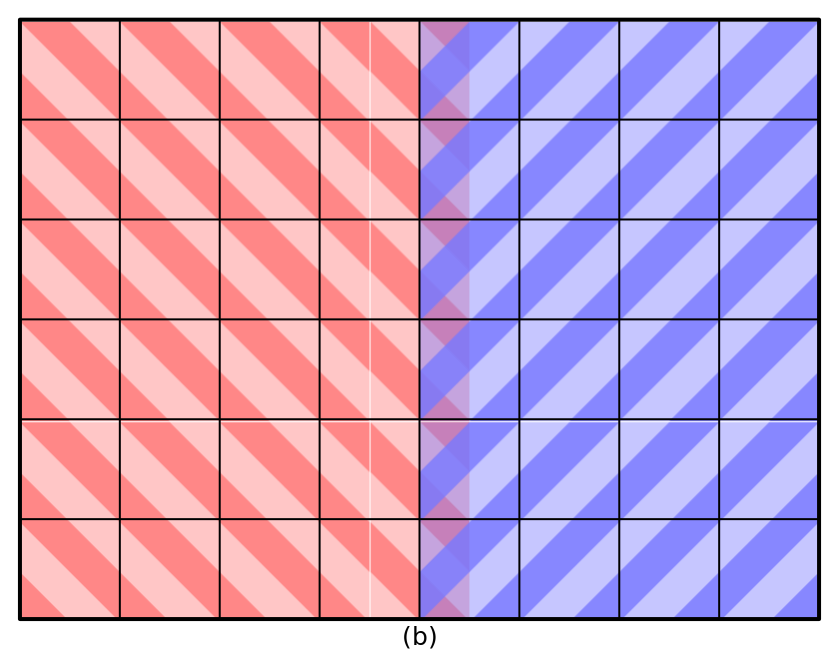
\includegraphics[width=0.40\textwidth]{img/fragmentos2.pdf}

	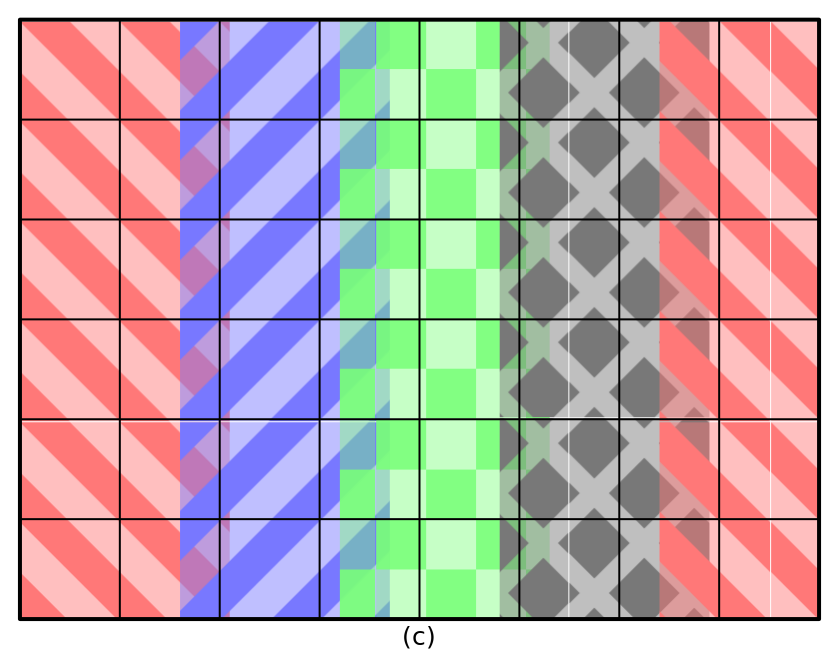
\includegraphics[width=0.40\textwidth]{img/fragmentos5.pdf}~
	
\includegraphics[width=0.40\textwidth]{img/fragmentos8.pdf}

\end{figure}

\end{frame}

\begin{frame}

\frametitle{Arquitectura del sistema}

\framesubtitle{Tareas del sistema}

\begin{itemize}

	\item Cada tarea estática tiene un hilo de ejecución.

	\item Existe un pool de hilos de ejecución para las tareas de búsqueda.

\end{itemize}

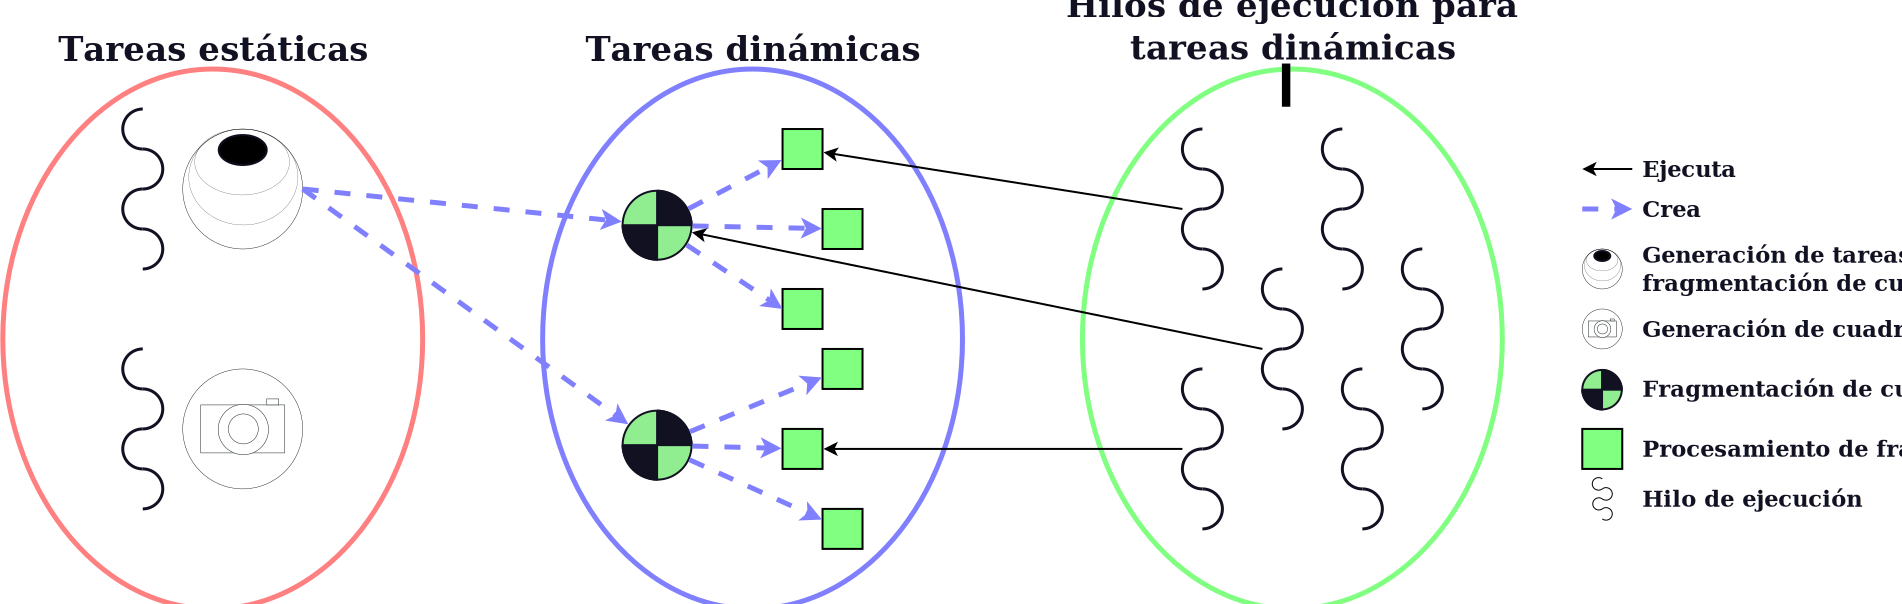
\includegraphics[width=\textwidth]{img/hilos.pdf}

\end{frame}

\begin{frame}

\frametitle{Arquitectura del sistema}

\framesubtitle{Flujo de los datos}

\begin{figure}[h]

	\centering

	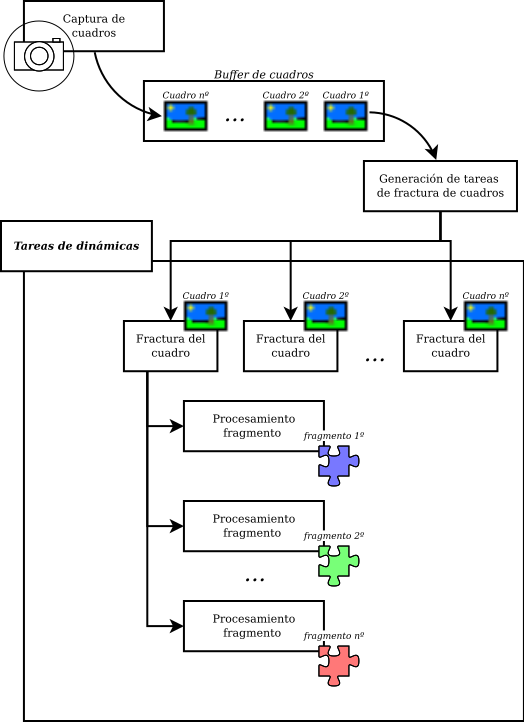
\includegraphics[height=0.95\textheight]{img/framework.pdf}

\end{figure}

\end{frame}

\begin{frame}

\frametitle{Experimentación}

Buscamos:

\begin{itemize}

	\item \emph{FPS} y luego Retardo de cuadro

\end{itemize}

Plataforma experimental:

\begin{itemize}

	\item Intel Xeon E5-2630 (2,3GHz) de 6 núcleos con multithreading
		simultáneo de dos vías (12 núcleos virtuales)

	\item Memoria cache 15MiB L3, 256KiB L2, 32KiB L1i, 32KiB L1d

\end{itemize}

Variables:

\begin{itemize}

	\item Dos vídeos 1280x720px y 800x600px.

	\item Cantidad de hilos para tareas dinámicas.

	\item de 1 a 12.

	\item Cantidad de fragmentos.

	\item de 1 a 24.

\end{itemize}

\end{frame}

\begin{frame}

\frametitle{Resultados: \emph{FPS} vídeo 1280x720px}

\includegraphics[width=\textwidth]{img/1280x720_fps.pdf}

\end{frame}

\begin{frame}

\frametitle{Resultados: \emph{FPS} números primos}

\includegraphics[width=\textwidth]{img/primos_fps.pdf}

\end{frame}

\begin{frame}

\frametitle{Resultados: \emph{FPS} vídeo 1280x720px}

\includegraphics[width=\textwidth]{img/1280x720_fps.pdf}

\end{frame}

\begin{frame}

\frametitle{Resultados: Fallos de cache por cuadro}

\includegraphics[width=\textwidth]{img/cache_fallos.pdf}

\end{frame}

\begin{frame}

\frametitle{Resultados}

\framesubtitle{FPS máximos}

\includegraphics[width=\textwidth]{img/1280x720_bestfps.pdf}

\end{frame}

\begin{frame}

\frametitle{Resultados}

\framesubtitle{Speedup}

\includegraphics[width=\textwidth]{img/1280x720_speedup.pdf}

\end{frame}

\begin{frame}

\frametitle{Retardo de cuadro por cada \emph{FPS}}

\includegraphics[width=\textwidth]{img/1280x720_tFPS.pdf}

\end{frame}

\begin{frame}

\frametitle{Usos educativos}

\framesubtitle{Para una cátedra de sistemas paralelos}

\begin{itemize}

	\item El sistema puede ser utilizado como practica para calcular el
		\emph{speedup} y eficiencia.
	
	\item Permite visualizar la importancia de la correcta fragmentación de
		los datos.

	\item Se puede experimentar con distintos requerimientos de \emph{FPS} y
		retardo de cuadro.

	\item Se pueden optimizar los plugins utilizando instrucciones
		vectoriales.

\end{itemize}

\end{frame}

\begin{frame}

\frametitle{Usos educativos}

\framesubtitle{Para una cátedra de visión por computadora}

\begin{itemize}

	\item Creación de nuevos plugins y pilas de plugins para la detección de
		nuevos objetos.

	\item Exploración de nuevos mecanismos de detección de los objetos.

	\item Adaptación del framework base a un nuevo dominio.

\end{itemize}

\end{frame}

\begin{frame}

\frametitle{Conclusiones}

\begin{itemize}

	\item Se desarrollo un sistema de visión global para fútbol de robots
		que puede ser utilizado como herramienta educativa.

	\item Se analizaron los comportamientos bajo distintas configuraciones,
		y se comprobó su desempeño.

\end{itemize}

Trabajos futuros:

\begin{itemize}

	\item Agregar una interfaz gráfica que permita visualizar los resultados
		de los plugins.

	\item Seguir trabajando sobre los plugins para hacerlos mas accesibles.

\end{itemize}

\end{frame}

\begin{frame}

	\frametitle{¡Muchas Gracias!}

\end{frame}

\bibliographystyle{babplain}

\bibliography{biblio}

\end{document}
